\section{Generování signálu}

Byl vygenerován signál obsahující pouze rušení složený z cosinusovek o frekvencích nalezených dříve pomocí funkce np.cos z knihovny numpy. Tento signál byl poté podroben spektrální analýze.
Výsledný signál byl normalizován a byl vytvořen spektrogram a spektrální hustota tohoto signálu.
Tento signál byl následně převeden na 16bit integer (pro uložení v 16bit wav) a uložen. Následně byl tento signál zobrazen v grafu.

\begin{figure}[H] 
	\centering
	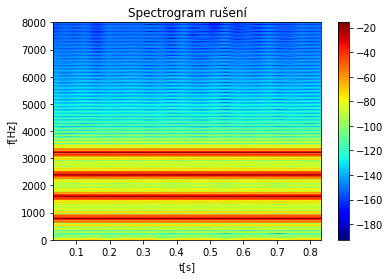
\includegraphics[scale=0.67,keepaspectratio]{Figure_8}
	\caption{Výkonový spektrogram rušení}
\end{figure}

\begin{figure}[H] 
	\centering
	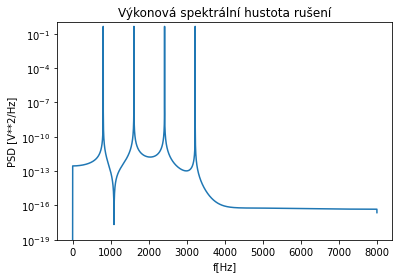
\includegraphics[scale=0.67,keepaspectratio]{Figure_9}
	\caption{Výkonová spektrální hustota rušení}
\end{figure}

\begin{landscape}
\begin{figure}[H] 
	\centering
	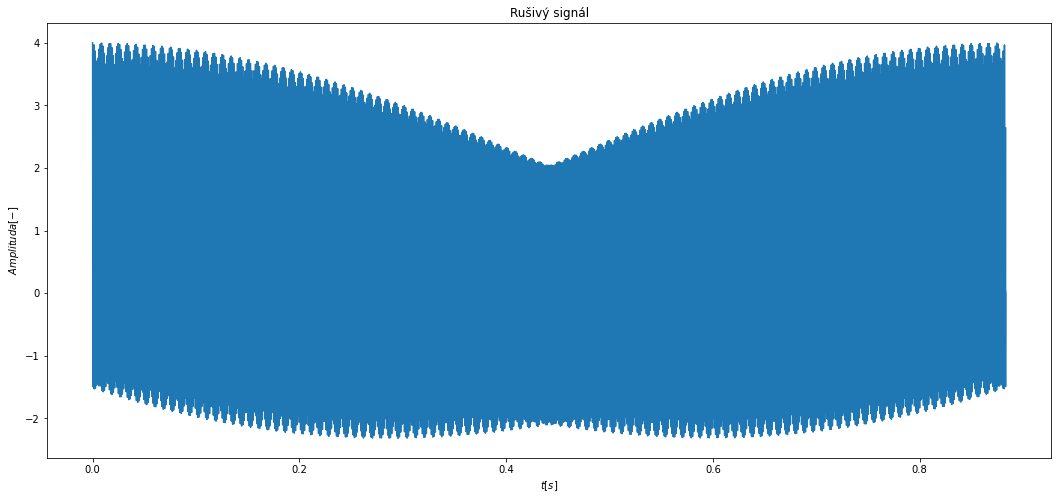
\includegraphics[scale=0.55,keepaspectratio]{Figure_25}
	\caption{Signál rušení}
\end{figure}
\end{landscape}